\chapter{Appendix}

\appendix \label{appendix}

\section{Traditional Feature-Based \ac{ser}}

\subsection{Audio Features Visualization} \label{app:1}

\begin{figure}[H]
	\centering
	\includegraphics[width=\linewidth]{figs/appendix/feature_selection/signalWP.png}
	\caption{Audio Signal wave plots of one audio segment for all emotions.}
	\label{fig:signalWP}
\end{figure}

\begin{figure}[H]
	\centering
	\includegraphics[width=\linewidth]{figs/appendix/feature_selection/melSpect.png}
	\caption{Log mel magnitude spectrograms of one audio segment for all emotions.}
	\label{fig:melSpect}
\end{figure}

\begin{figure}[H]
	\centering
	\includegraphics[width=\linewidth]{figs/appendix/feature_selection/mfccSpec.png}
	\caption{\ac{mcc} spectrogram of one audio segment for all emotions.}
	\label{fig:mfccSpec}
\end{figure}


\begin{figure}[H]
	\centering
	\includegraphics[width=\linewidth]{figs/appendix/feature_selection/ChromSpec.png}
	\caption{Chromogram spectrograms of one audio segment for all emotions.}
	\label{fig:ChromSpec}
\end{figure}

\begin{figure}[H]
	\centering
	\includegraphics[width=\linewidth]{figs/appendix/feature_selection/specWP.png}
	\caption{Spectral wave plots of one audio segment for all emotions.}
	\label{fig:SpecWP}
\end{figure}

\begin{figure}[H]
	\centering
	\includegraphics[width=\linewidth]{figs/appendix/feature_selection/rmseWP.png}
	\caption{Root-Mean-Square energy wave plots of one audio segment for all emotions.}
	\label{fig:rmseWP}
\end{figure}


\subsection{Features Mean Values Overview} \label{app:2}

\begin{figure}[H]
	\centering
	\includegraphics[width=\textwidth]{figs/appendix/feature_selection/meanSpectralFeatBarPlot.png}
	\caption{Bar plot with the mean values of the mean spectral centroid, bandwidth, roll-off, and contrast features.}
	\label{fig:meanSpectralFeatBarPlot}
\end{figure}

\begin{center}
	\begin{figure}[H]
		\centering
		\includegraphics[width=\linewidth]{figs/appendix/feature_selection/meanOtherFeatBarPlot.png}
		\caption{Bar plot with the mean values of the mean chromogram, root-mean-square and zero crossing rate features.}
		\label{fig:meanFeatBarPlot}
	\end{figure}
\end{center}


\subsection{Wave Plots with Surrounding Areas} \label{app:3}

\begin{figure}[H]
	\centering
	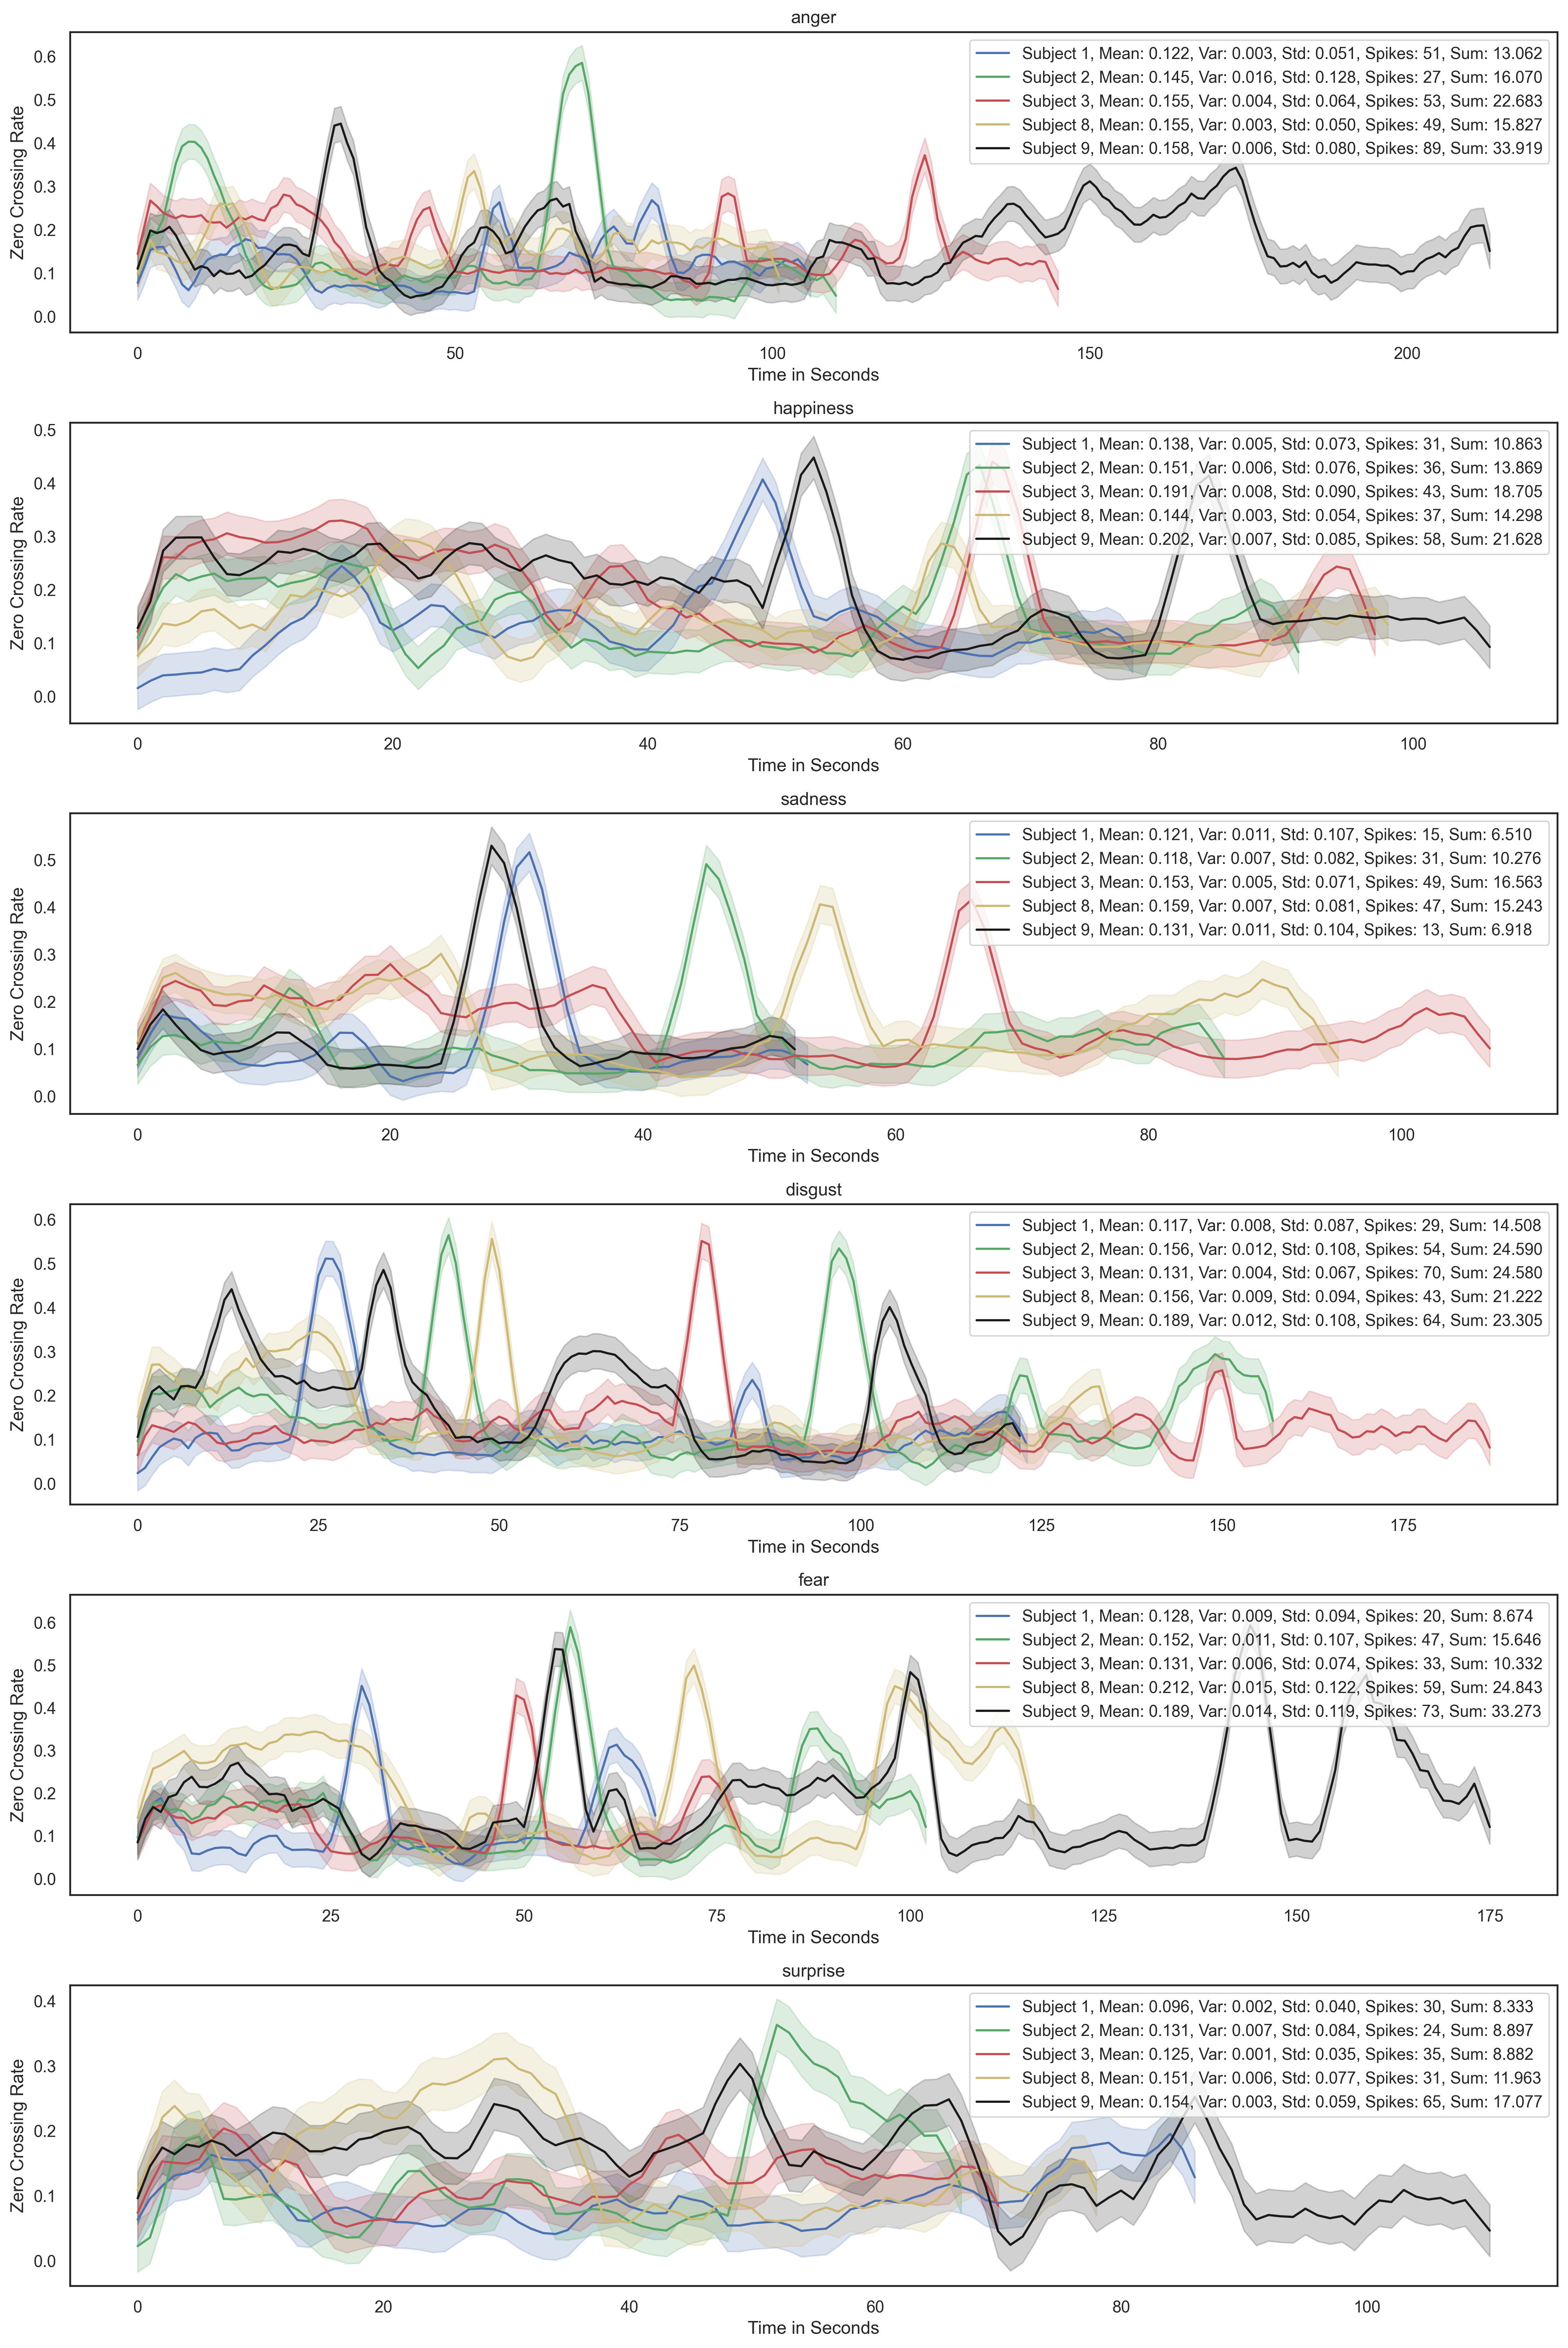
\includegraphics[width=\linewidth]{figs/appendix/feature_selection/zcrArea.png}
	\caption{Zero crossing rate wave plots with a surrounding area of five male subjects and the same sentence for all emotions.}
	\label{fig:zcrArea}
\end{figure}


\subsection{Variation Plots}  \label{app:4}

\begin{figure}[H]
	\centering
	\includegraphics[width=\linewidth]{figs/appendix/feature_selection/stdZCRVar.png}
	\caption{Zero crossing rate standard deviation values variation plot along 50 audios of speech utterances for all emotions.}
	\label{fig:stdZCRVar}
\end{figure}

\begin{figure}[H]
	\centering
	\includegraphics[width=\linewidth]{figs/appendix/feature_selection/spikesZCRVar.png}
	\caption{Zero crossing rate spikes values variation plot along 50 audios of speech utterances for all emotions.}
	\label{fig:spikesZCRVar}
\end{figure}

\begin{figure}[H]
	\centering
	\includegraphics[width=\linewidth]{figs/appendix/feature_selection/sumZCRVar.png}
	\caption{Zero crossing rate sum values variation plot along 50 audios of speech utterances for all emotions.}
	\label{fig:sumZCRVar}
\end{figure}


\subsection{Confusion Matrices}  \label{confusionMatrices}

\begin{figure}[H]
	\begin{subfigure}{.5\textwidth}
		\centering
		\includegraphics[width=\linewidth]{figs/appendix/feature_selection/cmAll.png}
		\caption{\ac{cm} using all 327 features.}
	\end{subfigure}%
	\begin{subfigure}{.5\textwidth}
		\centering
		\includegraphics[width=\linewidth]{figs/appendix/feature_selection/cmSec.png}
		\caption{\ac{cm} using 98 features after \ac{cfs}.}
	\end{subfigure}
	\newline
	\centering
	\begin{subfigure}{.5\textwidth}
		\centering
		\includegraphics[width=\linewidth]{figs/appendix/feature_selection/cmThird.png}
		\caption{\ac{cm} using 33 features after \ac{cfs} and backward selection.}
	\end{subfigure}
	\caption{\ac{rf} 5-fold \ac{cv} confusion matrices using different sets of features.}
\end{figure}


\subsection{Classifiers Evaluation and Selection} \label{app:5}


\begin{figure}[H]
	\begin{subfigure}{.5\textwidth}
		\centering
		\includegraphics[width=.9\linewidth]{figs/appendix/feature_selection/XGBoostCM.png}
		\caption{\ac{xgb} \ac{cm}.}
	\end{subfigure}%
	\begin{subfigure}{.5\textwidth}
		\centering
		\includegraphics[width=.9\linewidth]{figs/appendix/feature_selection/AdaBoostCM.png}
		\caption{AdaBoost \ac{cm}.}
	\end{subfigure}
	\newline
	\begin{subfigure}{.5\textwidth}
		\centering
		\includegraphics[width=.9\linewidth]{figs/appendix/feature_selection/BalancedForestCM.png}
		\caption{Balanced \ac{rf} \ac{cm}.}
	\end{subfigure}%
	\begin{subfigure}{.5\textwidth}
		\centering
		\includegraphics[width=.9\linewidth]{figs/appendix/feature_selection/RandomForestCM.png}
		\caption{\ac{rf} \ac{cm}.}
	\end{subfigure}
	\newline
	\begin{subfigure}{.5\textwidth}
		\centering
		\includegraphics[width=.9\linewidth]{figs/appendix/feature_selection/HistCM.png}
		\caption{Histogram Gradient Boosting \ac{cm}.}
	\end{subfigure}%
	\begin{subfigure}{.5\textwidth}
		\centering
		\includegraphics[width=.9\linewidth]{figs/appendix/feature_selection/SVMCM.png}
		\caption{\ac{svm} \ac{cm}.}
	\end{subfigure}
	\caption{Tested models' 5-fold stratified \ac{cv} confusion matrices on \ac{iemo} (1).}
\end{figure}

\begin{figure}[H]
	\begin{subfigure}{.5\textwidth}
		\centering
		\includegraphics[width=.9\linewidth]{figs/appendix/feature_selection/LDACM.png}
		\caption{Linear Discriminant Analysis \ac{cm}.}
	\end{subfigure}%
	\begin{subfigure}{.5\textwidth}
		\centering
		\includegraphics[width=.9\linewidth]{figs/appendix/feature_selection/RidgeCM.png}
		\caption{Ridge \ac{cm}.}
	\end{subfigure}
	\newline
	\begin{subfigure}{.5\textwidth}
		\centering
		\includegraphics[width=.9\linewidth]{figs/appendix/feature_selection/LSTMCM.png}
		\caption{\ac{lstm} \ac{cm}.}
	\end{subfigure}%
	\begin{subfigure}{.5\textwidth}
		\centering
		\includegraphics[width=.9\linewidth]{figs/appendix/feature_selection/CNNCM.png}
		\caption{\ac{cnn} \ac{cm}.}
	\end{subfigure}
	\caption{Tested models' 5-fold stratified \ac{cv} confusion matrices on \ac{iemo} (2).}
\end{figure}

\section{\acl{dl}-Based \ac{ser}}

\subsection{Classifiers Evaluation and Selection} \label{app:6}


\begin{figure}[H]
	\begin{subfigure}{.5\textwidth}
		\centering
		\includegraphics[width=.9\linewidth]{figs/appendix/feature_selection/ResSpec.png}
		\caption{Resnet50 using spectrogram images \ac{cm}.}
	\end{subfigure}%
	\begin{subfigure}{.5\textwidth}
		\centering
		\includegraphics[width=.9\linewidth]{figs/appendix/feature_selection/ResMelSpec.png}
		\caption{Resnet50 using mel spectrogram images \ac{cm}.}
	\end{subfigure}
	\newline
	\begin{subfigure}{.5\textwidth}
		\centering
		\includegraphics[width=.9\linewidth]{figs/appendix/feature_selection/ResMFCC.png}
		\caption{Resnet50 using \ac{mfccs} images \ac{cm}.}
	\end{subfigure}%
	\begin{subfigure}{.5\textwidth}
		\centering
		\includegraphics[width=.9\linewidth]{figs/appendix/feature_selection/VGGMelSpec.png}
		\caption{VGG16 using mel spectrogram images \ac{cm}.}
	\end{subfigure}
	\newline
	\begin{subfigure}{.5\textwidth}
		\centering
		\includegraphics[width=.9\linewidth]{figs/appendix/feature_selection/VGGMFCC.png}
		\caption{VGG16 using \ac{mfccs} images \ac{cm}.}
	\end{subfigure}%
	\begin{subfigure}{.5\textwidth}
		\centering
		\includegraphics[width=.9\linewidth]{figs/appendix/feature_selection/VGGSpec.png}
		\caption{VGG16 using spectrogram images \ac{cm}.}
	\end{subfigure}
	\caption{\ac{dl} classification models confusion matrices on \ac{iemo} (1).}
\end{figure}

\begin{figure}[H]
	\begin{subfigure}{.5\textwidth}
		\centering
		\includegraphics[width=.9\linewidth]{figs/appendix/feature_selection/XMelSpec.png}
		\caption{Xception using mel spectrogram images \ac{cm}.}
	\end{subfigure}%
	\begin{subfigure}{.5\textwidth}
		\centering
		\includegraphics[width=.9\linewidth]{figs/appendix/feature_selection/XMFCC.png}
		\caption{Xception using \ac{mfccs} images \ac{cm}.}
	\end{subfigure}
	\newline
	\begin{subfigure}{.5\textwidth}
		\centering
		\includegraphics[width=.9\linewidth]{figs/appendix/feature_selection/XSpec.png}
		\caption{Xception using spectrogram images \ac{cm}.}
	\end{subfigure}%
	\begin{subfigure}{.5\textwidth}
		\centering
		\includegraphics[width=.9\linewidth]{figs/appendix/feature_selection/CNNSpec.png}
		\caption{2D-\ac{cnn} using spectrograms \ac{cm}.}
	\end{subfigure}
	\newline
	\begin{subfigure}{.5\textwidth}
		\centering
		\includegraphics[width=.9\linewidth]{figs/appendix/feature_selection/LSTMMelSpec.png}
		\caption{2D-\ac{cnn} \& \ac{rnn} using mel spectrograms \ac{cm}.}
	\end{subfigure}%
	\begin{subfigure}{.5\textwidth}
		\centering
		\includegraphics[width=.9\linewidth]{figs/appendix/feature_selection/CNNMFCC.png}
		\caption{2D-\ac{cnn} using \ac{mfccs} \ac{cm}.}
	\end{subfigure}
	\caption{\ac{dl} classification models confusion matrices on \ac{iemo} (2).}
\end{figure}


\begin{figure}[H]
	\begin{subfigure}{.5\textwidth}
		\centering
		\includegraphics[width=.9\linewidth]{figs/appendix/feature_selection/LSTMSpec.png}
		\caption{2D-\ac{cnn} \& \ac{rnn} using spectrograms \ac{cm}.}
	\end{subfigure}%
	\begin{subfigure}{.5\textwidth}
		\centering
		\includegraphics[width=.9\linewidth]{figs/appendix/feature_selection/LSTMMFCC.png}
		\caption{2D-\ac{cnn} \& \ac{rnn} using \ac{mfccs} \ac{cm}.}
	\end{subfigure}
	\newline
	\centering
	\begin{subfigure}{.5\textwidth}
		\centering
		\includegraphics[width=.9\linewidth]{figs/appendix/feature_selection/CNNMelSpec.png}
		\caption{2D-\ac{cnn} using mel spectrograms \ac{cm}.}
	\end{subfigure}%
	\caption{\ac{dl} classification models confusion matrices on \ac{iemo} (3).}
\end{figure}

\section{Data Stratification}

\subsection{Dimensional Emotions} \label{app:7}

\begin{figure}[H]
	\centering
	\includegraphics[width=\linewidth]{figs/appendix/IEMOCAP_data_study/valenceScatterAllEmotions.png}
	\caption{Scatter plot of the annotated emotions in the valence dimension.}
\end{figure}


\begin{figure}[H]
	\centering
	\includegraphics[width=\linewidth]{figs/appendix/IEMOCAP_data_study/activationScatterAllEmotions.png}
	\caption{Scatter plot of the annotated emotions in the arousal dimension.}
\end{figure}

\begin{figure}[H]
	\centering
	\includegraphics[width=\linewidth]{figs/appendix/IEMOCAP_data_study/dominanceScatterAllEmotions.png}
	\caption{Scatter plot of the annotated emotions in the dominance dimension.}
\end{figure}


\begin{figure}[H]
	\centering
	\includegraphics[width=\linewidth]{figs/appendix/IEMOCAP_data_study/allScatterViolins.png}
	\caption{Scatter and violin plots of the emotional content of the \ac{iemo} in terms of \ac{vad} relative to the all emotions.}
\end{figure}

\begin{figure}[H]
	\centering
	\includegraphics[width=\linewidth]{figs/appendix/IEMOCAP_data_study/angryScatterViolins.png}
	\caption{Scatter and violin plots of the emotional content of the \ac{iemo} in terms of \ac{vad} relative to the angry emotion.}
\end{figure}


\begin{figure}[H]
	\centering
	\includegraphics[width=\linewidth]{figs/appendix/IEMOCAP_data_study/happyScatterViolins.png}
	\caption{Scatter and violin plots of the emotional content of the \ac{iemo} in terms of \ac{vad} relative to the happiness emotion.}
\end{figure}


\begin{figure}[H]
	\centering
	\includegraphics[width=\linewidth]{figs/appendix/IEMOCAP_data_study/sadScatterViolins.png}
	\caption{Scatter and violin plots of the emotional content of the \ac{iemo} in terms of \ac{vad} relative to the sad emotion.}
\end{figure}

\begin{figure}[H]
	\centering
	\includegraphics[width=\linewidth]{figs/appendix/IEMOCAP_data_study/neutralScatterViolins.png}
	\caption{Scatter and violin plots of the emotional content of the \ac{iemo} in terms of \ac{vad} relative to the neutral emotion.}
\end{figure}

